% !TeX spellcheck = it_IT
% !TeX root = thesis-main.tex
\documentclass[12pt,a4paper,openright,twoside]{book}
\usepackage[utf8]{inputenc}
\usepackage[italian]{babel}
\usepackage[hyperfootnotes=false]{hyperref}
\usepackage{disi-thesis}
\usepackage[acronym,toc]{glossaries}
\usepackage{code-lstlistings}
\usepackage{notes}
\usepackage{shortcuts}
\usepackage{float}
\usepackage{pgfplots}

\newcommand{\acknowledgementsname}{Riconoscimenti}
\renewcommand{\chaptername}{Capitolo} % Per i capitoli
\renewcommand{\bibname}{Bibliografia} % Per la bibliografia
\renewcommand{\contentsname}{Indice}  % Per il sommario
\renewcommand{\listfigurename}{Elenco delle figure}
\renewcommand{\listtablename}{Elenco delle tabelle}

\glsdisablehyper

\pagenumbering{roman}



\school{\unibo}
\programme{Corso di Laurea in Ingegneria e Scienze Informatiche}
\title{ClientShield: Implementazione di un Servizio Windows per la Sicurezza DNS}
\author{Federico Diotallevi}
\date{\today}
\subject{Programmazione ad Oggetti}
\supervisor{Prof.\ Viroli Mirko}
%\cosupervisor{Nicolas Farabegoli}
\session{IV}
\academicyear{2023\ -\ 2024}

\newacronym{DoH}{DoH}{DNS over HTTPS}
\newacronym{DNS}{DNS}{Domain Name System}
\newacronym{AI}{AI}{Intelligenza Artificiale}
\newacronym{PoC}{PoC}{Proof of Concept}
\newacronym{AGID}{AGID}{Agenzia per l'Italia Digitale}
\newacronym{VPN}{VPN}{Virtual Private Network}
\newacronym{HTTPS}{HTTPS}{HTTP Secure}
\newacronym{ISP}{ISP}{Internet Service Provider}


\mainlinespacing{1.241} % line spacing in mainmatter, comment to default (1)

\begin{document}

\frontmatter\frontispiece\

\renewcommand{\abstractname}{Sommario}
\begin{abstract}

Lo sviluppo della tecnologia cresce sempre più velocemente e, con essa, anche i rischi che gli utenti corrono semplicemente navigando in rete.
Questa tesi si inserisce nell'ambito dell'internet filtering, cioè la possibilità di filtrare il traffico in rete negando l'accesso a siti potenzialmente pericolosi.

L'obiettivo di questo progetto è lo sviluppo di un software che sia facilmente installabile su un dispositivo Windows e filtri tutte le richieste web effettuate.
Si vuole offrire la possibilità ad un un amministratore di rete di attivare e disattivare la protezione del dispositivo da remoto, decidendo eventualmente anche quali categorie di siti bloccare.

Per lo sviluppo è stata fondamentale la collaborazione con FlashStart, azienda di riferimento nel mercato italiano per quanto riguarda il filtraggio \gls{DNS}.

Il software è stato sviluppato in contesto aziendale come prototipo e sfrutta ampiamente le soluzioni di filtraggio aziendali.
Ciò ha facilitato la gestione delle categorie e dell'effettivo filtraggio \gls{DNS}, permettendo al progetto di focalizzarsi sulla cattura e redirezione del traffico internet del dispositivo verso i server gestiti da FlashStart.
\end{abstract}

\begin{dedication}
Optional dedication.
\end{dedication}

%----------------------------------------------------------------------------------------
\tableofcontents   
%\listoffigures     % (optional) comment if empty
%\lstlistoflistings\ % (optional) comment if empty
%----------------------------------------------------------------------------------------

%----------------------------------------------------------------------------------------
\chapterWithoutNumber{Introduzione}
\phantomsection % to makr label work
\label{chap:introduzione}
%----------------------------------------------------------------------------------------

Navigare in rete è senz'altro una delle attività più diffuse al giorno d'oggi in tutto il mondo.
La quantità di informazioni a cui si può accedere è pressoché infinita e, soprattutto, a disposizione di chiunque.

La digitalizzazione delle risorse è ormai diventata essenziale per qualsiasi realtà, dal settore pubblico a quello privato.
Tuttavia, tale pratica espone inevitabilmente al rischio che documenti,
dati e informazioni sensibili diventino obiettivo di attacchi informatici.
A conferma di ciò, il recente rapporto \cite{clusit2024-sicurezza} evidenzia come gli attacchi informatici gravi a livello globale siano passati,
in media, da 4.5 a 9 al giorno in soli cinque anni.
Secondo il rapporto, gli incidenti critici sono aumentati dal 47\% all'81\% del totale e,
in Italia, il 58\% degli attacchi è costituito da malware, phishing e social engineering.

Con il recente e rapidissimo sviluppo dell' \gls{AI} il campo dell'Internet Filtering ha subito un vera e propria rivoluzione.
I nuovi modelli di Machine Learning sono capaci di analizzare e identificare con precisione siti malevoli,
grazie anche ai giganteschi volumi di dati di cui dispongono.
Questi sistemi riescono a riconoscere tecniche di phishing e malware avanzate, anche quando progettate per eludere i metodi di rilevamento tradizionali.

Questa tesi si colloca in questo contesto e si propone l'obiettivo di sviluppare un software prototipale per il filtraggio internet sul computer di installazione.
Il lavoro illustrerà dettagliatamente tutte le fasi di analisi, progettazione e sviluppo del progetto.

Data la necessità di interazione con componenti specifici del sistema operativo,
il software è stato sviluppato esclusivamente per Windows, con l'obiettivo di creare un servizio di sistema.

\paragraph{Struttura della Tesi}

La tesi si articola in 4 capitoli principali, che descrivono le diverse fasi della realizzazione del progetto, in particolare:

\begin{itemize}

    \item \textbf{Capitolo 1 (Contesto)}: in questo capitolo si tratta in maniera approfondita il problema affrontato dalla tesi.
    Viene analizzato il software attualmente presente in FlashStart e le motivazioni che inducono alla necessità di un nuovo sviluppo.
    
    \item \textbf{Capitolo 2 (Requisiti)}: in questo capitolo vengono affrontati casi d'uso e requisiti, analizzando il funzionamento e la percezione del progetto dal punto di vista dell'utente.
    
    \item \textbf{Capitolo 3 (Tecnologie)}:
    in questo capitolo vengono riportate le diverse tecnologie utilizzate e le scelte che hanno portato al loro impiego nel progetto.
    
    \item \textbf{Capitolo 4 (Analisi e progettazione)}:
    in questo capitolo viene descritta la fase di analisi e progettazione del sistema,
    illustrandone in particolare l'architettura e i pattern utilizzati, evidenziando in che modo il software ne tragga guadagno.

\end{itemize}

\mainmatter

\chapter{Contesto}
\label{chap:contesto}

\section{Internet Filtering}

Il caso di studio oggetto di questa tesi è un software prototipale, che si inserisce nell'ambito dell'Internet Filtering.
Per Internet Filtering si intende un sistema di monitorazione, controllo e limitazione dell'accesso alle risorse online, basato su criteri predefiniti.

Una tecnologia di questo tipo risulta particolarmente utile ad aziende, scuole ed enti pubblici.
Tramite questa pratica è infatti possibile effettuare controlli sul contenuto delle pagine web, limitando o impedendo l'accesso a siti contenenti malware o, eventualmente, contenuti indesiderati (ad esempio siti di scommesse, pornografia, droghe...).
Risulta evidente fin da subito che, per garantire un filtraggio di contenuti preciso ed efficace, sia necessaria un'attenta analisi delle pagine web, evitando di correre il rischio di impedirne immotivatamente l'accesso.

Questa tesi è svolta come progetto in collaborazione con FlashStart, leader italiana per quanto riguarda il filtraggio \gls{DNS}.
Un server \gls{DNS} è un sistema che permette di tradurre nomi di domini leggibili da un uomo, in indirizzi interpretabili da dei computer per connettersi tra loro.
Il filtraggio si basa proprio su questo principio: quando si accede ad un sito web attraverso un browser qualsiasi, il computer interrogherà un server \gls{DNS} per ottenere l'indirizzo attraverso cui sia possibile accedere al sito.
Con un'apposita configurazione, si può indurre il \gls{DNS} a bloccare la risoluzione di pagine web malevoli o riportanti contenuti non graditi.
FlashStart offre un servizio \gls{DNS} configurabile, attraverso cui è possibile definire delle categorie di contenuti da bloccare.
I server dell'azienda aggiornano continuamente la lista delle categorie bloccate, facendo largo uso di \gls{AI} per garantire rapido aggiornamento (in risposta alla nascita di nuovi siti) ed alta precisione.
Quando un utente, utilizzando un computer protetto dal servizio di FlashStart, tenta di accedere ad un sito appartenente ad una delle categorie bloccate, il \gls{DNS} risponderà alla richiesta di risoluzione del nome con l'indirizzo di una pagina indicante i motivi del blocco, al posto di quella richiesta.

\section{Obiettivi del Progetto}
\label{sec:obiettivi-progetto}

Il filtraggio \gls{DNS} può essere implementato in diverse modalità, di seguito le principali:

\begin{itemize}
	\item \textbf{A livello di rete:} applicato direttamente dall'\gls{ISP}\footnote{
		Un \gls{ISP} è un fornitore che offre connettività alla rete, consentendo ai suoi utenti di accedere a Internet. Gli ISP possono anche fornire servizi aggiuntivi, come, appunto, sicurezza informatica e filtraggio.}, blocca l'accesso a domini malevoli prima che le richieste raggiungano la rete locale.  
	\newline \textit{Esempio: un'azienda utilizza un servizio \gls{DNS} filtrato fornito dal proprio \gls{ISP} per impedire l'accesso a siti malevoli su tutta la rete aziendale.}
	
	\item \textbf{A livello di router:} il router funge da punto di controllo, utilizzando un server DNS con filtraggio per impedire l'accesso a contenuti non autorizzati. Tutti i dispositivi connessi alla rete collegata al router beneficiano automaticamente della protezione.
	\newline \textit{Esempio: un istituto scolastico configura il proprio router con un DNS appositamente configurato per impedire l'accesso a siti per adulti e social network bloccandoli per gli studenti.}
	
	\item \textbf{A livello di endpoint:} il filtraggio DNS è applicato direttamente sui dispositivi tramite configurazione manuale o software specifici, garantendo protezione anche fuori dalla rete aziendale o domestica.  
	\newline \textit{Esempio: un dipendente che lavora da remoto utilizza un client DNS sicuro sul proprio laptop per proteggersi dalle minacce.}
\end{itemize}

FlashStart offre prodotti per tutte le suddette modalità, tuttavia questo progetto prende in esame soltanto la terza tipologia di protezione \gls{DNS}, ossia il filtraggio a livello di endpoint.
Nel periodo tra il 2019 e il 2021 le aziende italiane, così come quelle di tutto il mondo, hanno dovuto affrontare la necessità dell'impiego del lavoro remoto.
Se da una parte tale pratica rappresenta un'opportunità per i lavoratori, che ne guadagnano in flessibilità, dall'altra espone l'azienda a nuovi rischi.
A dimostrazione di ciò, proprio nel 2020 è stato emanato dall'\gls{AGID} il vademecum \cite{AgID2020}, cioè una serie di undici raccomandazioni che offrono linee guida per garantire la sicurezza del lavoro da remoto.

In effetti, un dispositivo che esce dall'azienda, ambiente potenzialmente controllato e protetto, diventa un rischio.
Un dipendente potrebbe involontariamente navigare in siti di phishing e malware o connettersi a reti Wi-Fi infette, esponendo l'azienda al rischio di furti o compromissione di dati.
Obiettivo fondante di questa tesi è lo sviluppo di un software facilmente installabile su un computer Windows, che consenta una protezione efficace e completa ai dispositivi desktop che escono dalla rete aziendale.
Tale progetto dovrà filtrare la connessione dell'endpoint remoto, bloccando l'accesso a siti pericolosi, come virus e frodi, ma anche a contenuti indesiderati e distrazioni sul lavoro, come social network o videogiochi.

\section{Contesto Aziendale}

FlashStart offre già un software di protezione da malware e contenuti indesiderati dedicato ad endpoint remoti: ClientShield.
Tale prodotto rappresenta un'estensione del filtro aziendale, fornendo lo stesso tipo di protezione, configurabile attraverso la medesima piattaforma cloud da parte di un amministratore di rete.

Allo stato dell'arte il prodotto utilizza una \gls{VPN}, per stabilire una comunicazione sicura con i server di FlashStart.
Ciò garantisce che il dispositivo possa inviare e ricevere non soltanto le informazioni sul prodotto, ma anche richieste \gls{DNS}, generalmente trasmesse in chiaro, in modo totalmente criptato.

L'esigenza di aggiornamento del software deriva dalla volontà di FlashStart di integrare il protocollo \gls{DoH}, descritto in \cite{RFC8484}, nei suoi prodotti.
Rispetto ad una classica \gls{VPN}, \gls{DoH} sfrutta la crittografia asimmetrica, implementata dal protocollo \gls{HTTPS}, per garantire autenticazione, confidenzialità e integrità delle richieste \gls{DNS}.

Il vantaggio che FlashStart trae da entrambi i protocolli è essenzialmente il medesimo: proteggere le comunicazioni \gls{DNS} tramite la crittografia, evitando la possibilità di attacchi dovuti alla trasparenza delle informazioni.
La differenza principale tra i due approcci è che una \gls{VPN} cripta il traffico di rete nella sua interezza, mascherando anche l'indirizzo IP del dispositivo, mentre \gls{DoH} si concentra esclusivamente sulla protezione delle richieste \gls{DNS}.

Per un'azienda come FlashStart, specializzata in filtraggio \gls{DNS}, mascherare l'indirizzo IP di un endpoint non è una funzionalità totalmente rilevante per l'erogazione del suo servizio.
L'adozione del protocollo \gls{DoH} consente quindi di ottenere la riservatezza necessaria per la comunicazione con il \gls{DNS}, eliminando la necessità di un'infrastruttura \gls{VPN} dedicata e riducendo l'overhead complessivo del sistema.

La novità principale del software prototipale illustrato in questa tesi, è dunque quella di fornire una soluzione per la transizione dalla tecnologia \gls{VPN}, all'adozione del protocollo \gls{DoH}.
Di fondamentale importanza è inoltre l'analisi e la valutazione di soluzioni architetturali atte a garantire la naturale evoluzione del software, facilitando l'introduzione di nuove funzionalità.

\chapter{Analisi dei Requisiti}

\section{Scopo del sistema e analisi del dominio}

L'analisi del dominio è un punto chiave per quanto riguarda lo sviluppo software.
Tale fase permette di comprendere il contesto in cui il software opera, gli attori principali ed i loro scopi.
In questo progetto l'analisi del dominio è risultata molto rapida e diretta, in quanto il prodotto è stato sviluppato con un'azienda del settore informatico, permettendo fin da subito l'utilizzo di un linguaggio tecnico.

Come già introdotto nella sezione \ref{sec:obiettivi-progetto}, il contesto in cui opera l'applicazione è quello della sicurezza informatica.
Il fine ultimo di ClientShield è di fornire una soluzione di filtraggio \gls{DNS} avanzata, che consenta un'efficace protezione ad un dispositivo che naviga al di fuori di una rete protetta.
L'interazione col software coinvolgerà in particolare:

\begin{itemize}
	\item \textbf{Utente finale:} cioè l'utilizzatore del dispositivo da proteggere, il quale navigherà normalmente in internet, utilizzando un browser ed inviando naturalmente richieste \gls{DNS}.
	
	\item \textbf{Amministratore di rete:} il cliente FlashStart, responsabile dell'installazione e configurazione del software sul dispositivo attraverso la chiave fornita sulla piattaforma cloud. 
	Tramite l'applicativo online potrà gestire le policy di filtraggio, aggiungendo o rimuovendo siti specifici o intere categorie di contenuti da bloccare.

	\item \textbf{Server FlashStart:} riceveranno le richieste \gls{DNS} effettuate dal dispositivo protetto e le risolveranno applicando i filtri configurati dall'amministratore di rete.
\end{itemize}
Il software dovrà operare in modo tale da rendersi completamente trasparente all'utente finale, il quale non dovrebbe percepire alcuna differenza durante la normale navigazione. L'unico momento in cui sarà consapevole della presenza di un filtro, sarà durante il tentativo di accesso ad un contenuto online bloccato, in tal caso visualizzerà invece una schermata di blocco riportante eventualmente le motivazioni.

\section{Requisiti funzionali}

Il progetto prevede lo sviluppo di un'implementazione prototipale, ciò implica che le funzionalità del software trattate in questa tesi rappresentino un sottogruppo delle capacità che dovrà avere il sistema.
Tuttavia, poiché il risultato dello studio mira a gettare delle solide basi per una futura implementazione business di ClientShield, di seguito verranno elencati i requisiti del software nella sua interezza.
Una visione complessiva, infatti, permette di valutare fin da subito la possibilità di una futura integrazione delle funzioni aggiuntive, consentendo un'analisi più efficace.

Nella sua implementazione prototipale, ClientShield dovrà:

\begin{itemize}
	\item \textbf{Redirezionare le richieste \gls{DNS}:}
	l'applicazione catturerà tutto il traffico \gls{DNS} del dispositivo su cui è installata.
	Tutte le richieste devono essere redirezionate ai server FlashStart, sfruttando il protocollo \gls{DoH}.
	La risoluzione dei domini deve essere effettuata dai server aziendali, ClientShield agirà da client \gls{DoH}, facendo in modo di impedire la possibilità di \gls{DNS} leak\footnote{\textbf{DNS leak} si verificano quando le richieste \gls{DNS} non sono cifrate e vengono trasmesse in chiaro.  
		In questa condizione, un attaccante o qualsiasi entità che intercetti il traffico può monitorare i siti visitati dall'utente, compromettendo la privacy della navigazione.}.

	
	\item \textbf{Permettere la registrazione di un dispositivo localmente:}
	dopo l'installazione del software, chiunque disponga di una valida chiave di registrazione, può registrare il dispositivo.
	Per effettuare tale operazione saranno richiesti:
	\begin{itemize}
		\item \textit{chiave di registrazione:} ottenibile tramite un profilo cloud con la corretta licenza.
		\item \textit{nome del dispositivo:} una qualsiasi stringa che faciliti l'identificazione dell'endpoint ad un amministratore di rete.
	\end{itemize}
	Al termine della fase di registrazione, se avvenuta con successo, la protezione dovrà essere attivata e il dispositivo sarà visibile sulla piattaforma cloud.
	
	
	\item \textbf{Permettere abilitazione/disabilitazione della protezione localmente:}
	accedendo all'applicazione, qualora la protezione sia disattivata, si dovrà offrire la possibilità di attivarla.
	Viceversa, se la protezione è attiva, l'utente avrà la possibilità di disattivarla inserendo un PIN.
	Tale codice è un numero intero presente sulla piattaforma cloud e dunque visualizzabile soltanto da un amministratore di rete.
	
	\item \textbf{Controllare lo stato:}
	l'applicazione dovrà periodicamente connettersi ai server FlashStart per verificare lo stato della protezione.
	Questa operazione nell'implementazione prototipale, ha la funzione di verificare che il dispositivo sia ancora registrato sul cloud.
	La cancellazione dell'endpoint attraverso la piattaforma cloud, determinerà la disattivazione della protezione e la richiesta di una nuova registrazione.
	
	\item \textbf{Attivarsi automaticamente al riavvio:}
	se l'endpoint è già stato registrato, l'applicazione dovrà garantire il corretto funzionamento della protezione anche al riavvio.
	Ciò vuol dire che, all'accensione del dispositivo non dovrà essere necessaria, una nuova registrazione.
	ClientShield ricorderà le credenziali attive prima dello spegnimento, riattivando automaticamente la protezione all'accensione con le stesse.
	
\end{itemize}
Queste funzionalità costituiscono il complessivo comportamento del prototipo sviluppato in questo progetto.
L'obiettivo essenziale è dunque garantire la protezione del dispositivo, fungendo da intermediario tra l'endpoint e i server di FlashStart.

Con lo scopo di descrivere in modo semplice l'interazione tra utente, ClientShield e server \gls{DNS} FlashStart è stato realizzato il digramma di in figura \ref{fig:interazione-utente-software-server}.

\begin{figure}[H]
	\centering
	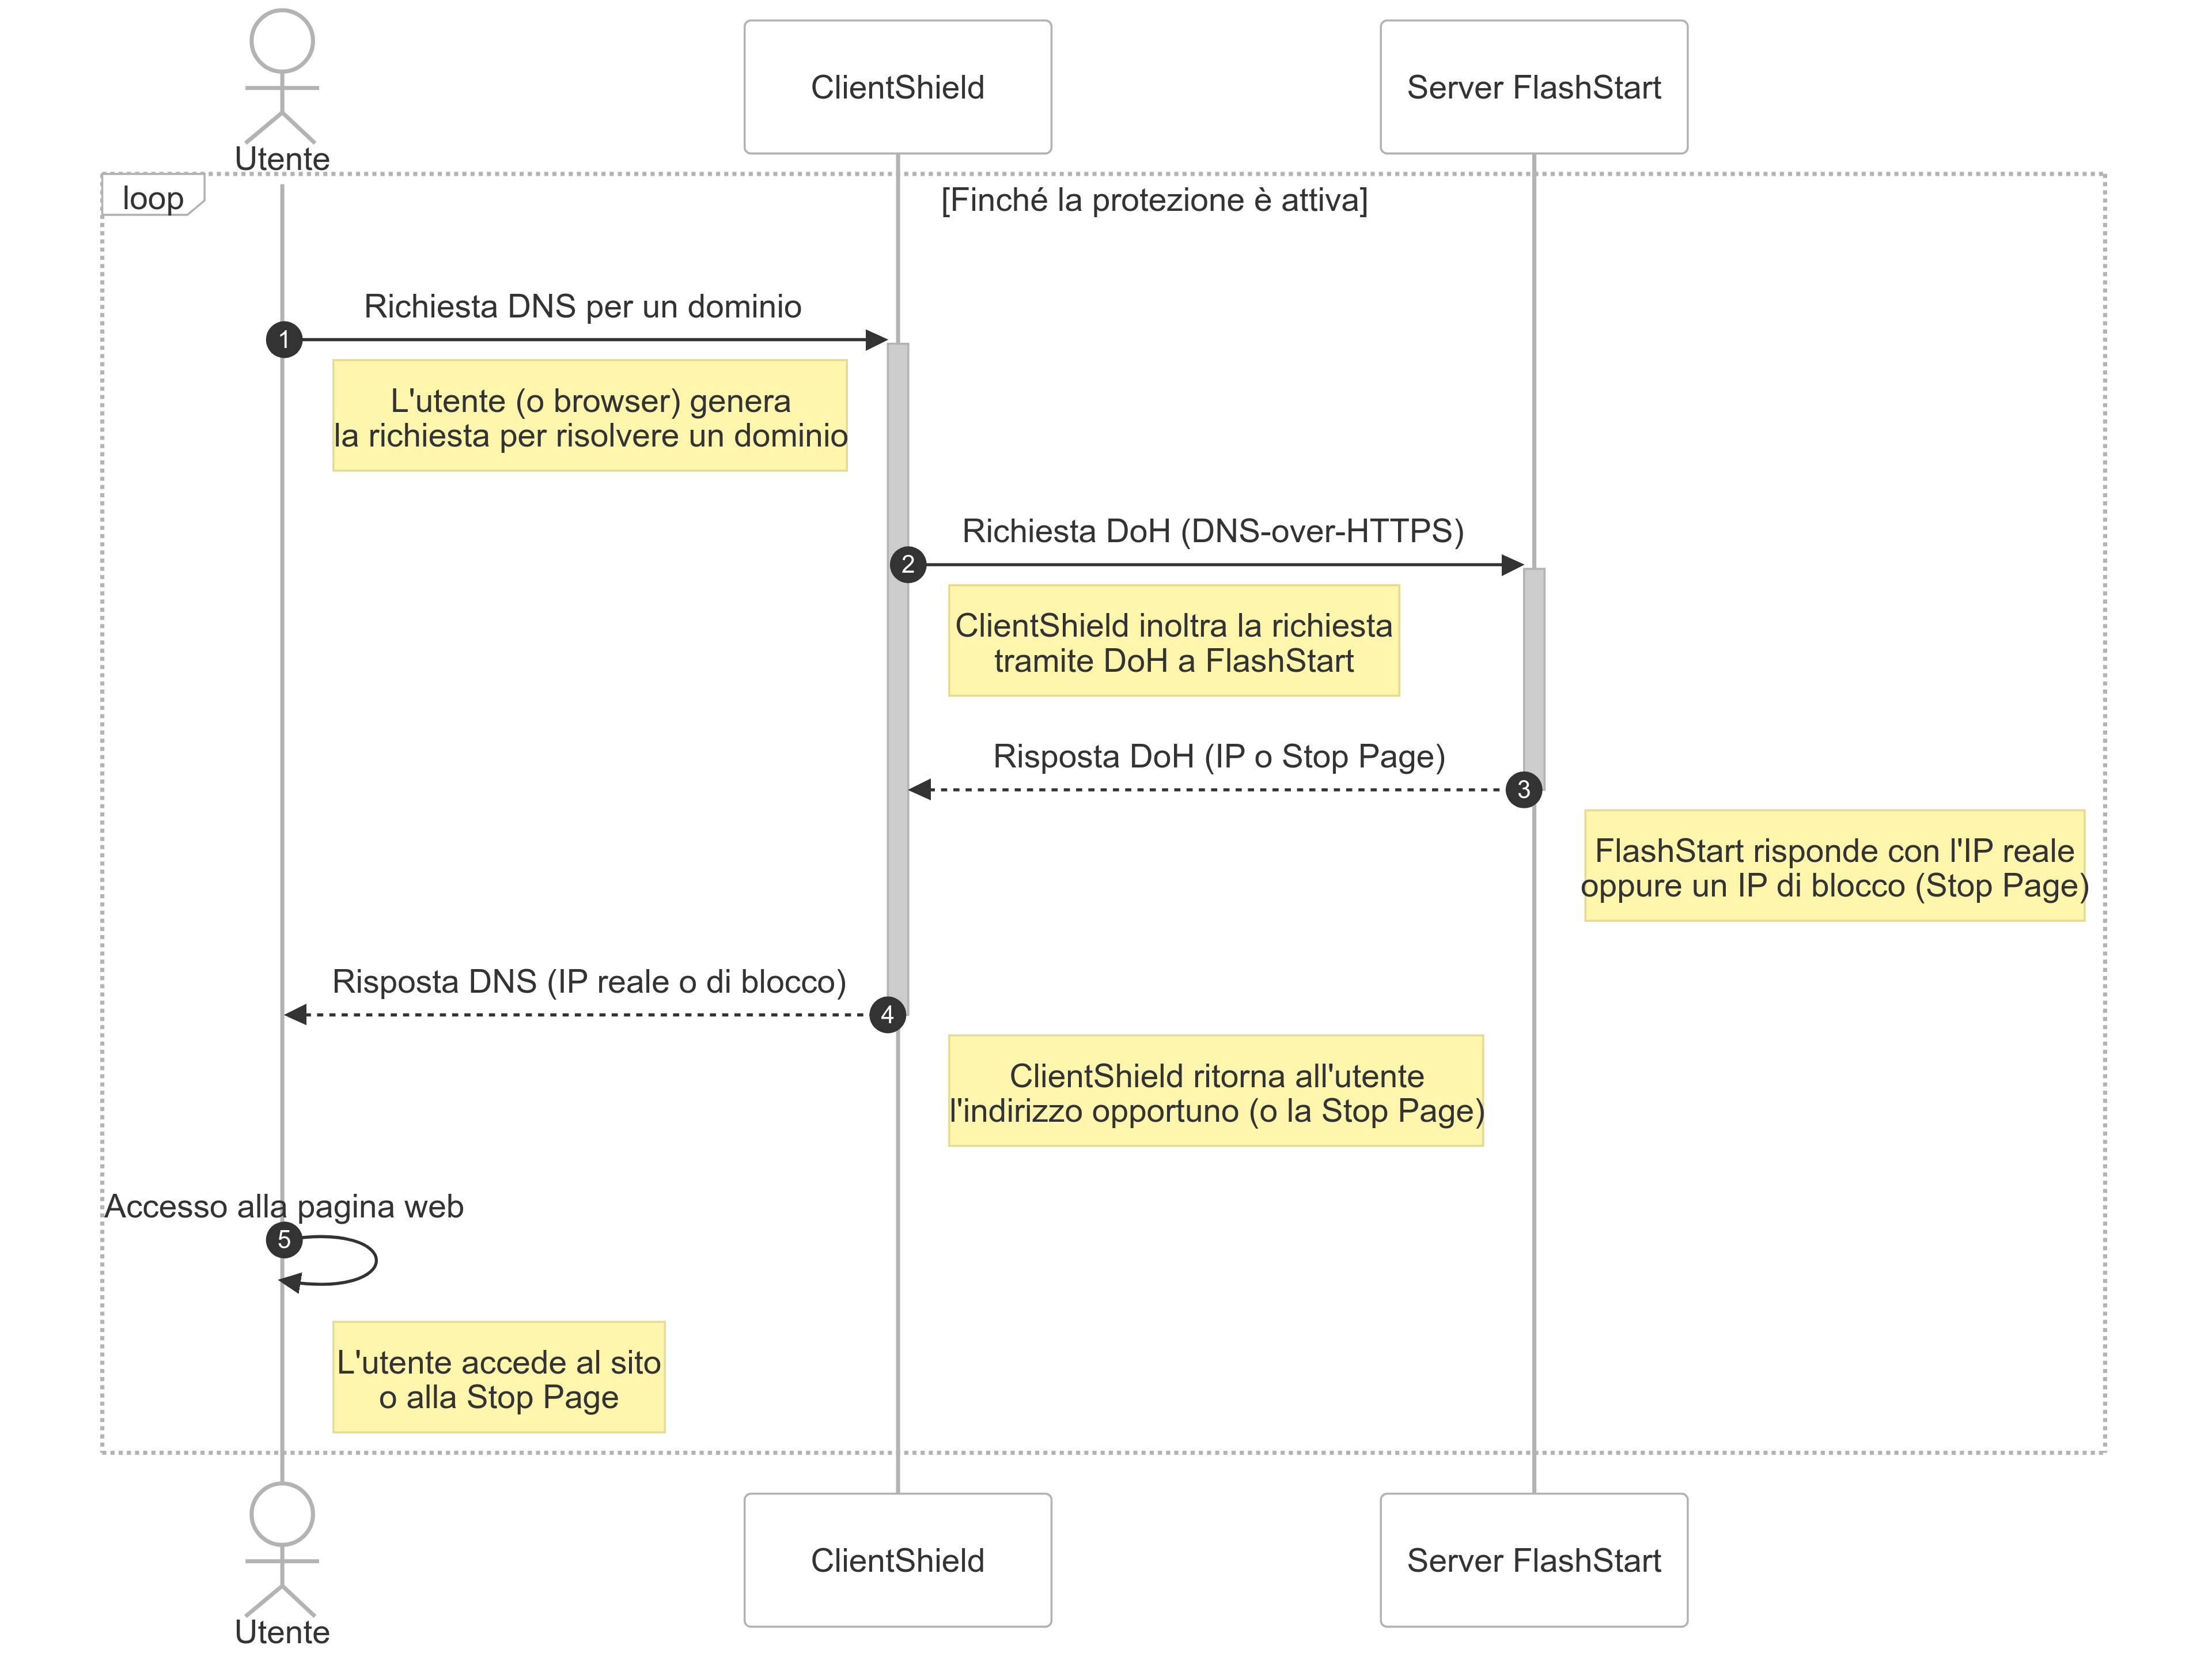
\includegraphics[width=1.0\textwidth]{figures/schema-utente-software-server.png}
	\caption{interazione tra utente, software e server FlashStart}
	\label{fig:interazione-utente-software-server}
\end{figure}
Come precedentemente anticipato, la versione business dell'applicazione garantirà una serie di funzioni minori in più, di seguito riportate:

\begin{itemize}
	
	\item \textbf{Blocco remoto della protezione:}
	deve essere possibile disattivare la protezione da remoto, questa funzione può essere utilizzata sia dall'amministratore di rete, attraverso la piattaforma cloud, sia direttamente dai server FlashStart.
	Durante i controlli di stato periodici, infatti, verrà verificata la validità della licenza e, se non risultasse valida, la protezione verrà disattivata automaticamente, impedendo qualsiasi tentativo di riattivazione locale.
	
	\item \textbf{Invio di notifiche:}
	durante la registrazione sarà possibile decidere di ricevere alcune notifiche dall'applicazione.
	Se attivate, il dispositivo riceverà soltanto le notifiche riguardanti lo stato della protezione del dispositivo, ad esempio licenza scaduta o disabilitazione remota.
	
	\item \textbf{Applicazione unbranded:}
	l'applicazione prima della registrazione dovrebbe avere un nome generico e non presentare alcun logo.
	Dopo la registrazione dovrà essere possibile ottenere informazioni sull'acquirente, come il nome scelto per il software e il logo da applicare.
	L'interfaccia grafica dell'applicazione dovrà adattarsi alle informazioni ottenute durante la registrazione.
	
	\item \textbf{Controllo di stato periodico:}
	questa operazione è già presente in parte nell'implementazione prototipale, tuttavia nello sviluppo business dovrà reperire più informazioni.
	I dati supplementari, come ad esempio:
	\begin{itemize}
		\item informazioni sul blocco remoto
		\item nome e logo dell'acquirente
		\item cambio di impostazioni sulle notifiche
	\end{itemize}
	permetteranno l'implementazione delle funzionalità aggiuntive sopra riportate

\end{itemize}
Come si può notare, le funzionalità business rappresentano più che altro un'estensione di funzioni già presenti nel modello prototipale.
Con una corretta analisi del software, dunque, dovrebbe essere possibile aggiungere tutte le funzionalità supplementari al sistema descritto in questa tesi senza particolari sforzi.

\section{Requisiti non funzionali}

Dopo aver definito in dettaglio \textit{cosa} deve fare ClientShield, è altrettanto importante stabilire \textit{come} debba farlo.
Oltre ai requisiti funzionali del sistema, infatti, il progetto prevede anche dei requisiti non funzionali, che mirano a garantire un livello qualitativo adeguato al sistema.
Questa categoria di requisiti ha l'obiettivo di soddisfare un potenziale cliente.
L'aderenza ad essi dovrebbe trasmettere la professionalità di FlashStart, garantendo un'esperienza di utilizzo piacevole per gli utilizzatori finali.

\subsection*{Semplicità}

Di fondamentale importanza è rendere il sistema semplice: rapido da installare e facile da configurare.  
FlashStart ha esplicitamente sottolineato quanto questo requisito sia cruciale per garantire la qualità del software.
La richiesta è naturalmente intuitiva: un'installazione e una configurazione rapide non solo migliorano l’esperienza dell’utente, ma rendono il software più facilmente integrabile nei diversi contesti aziendali.  
L'automatizzazione completa del processo di installazione consente agli amministratori di rete di implementare ClientShield senza difficoltà, ottimizzando i tempi e riducendo il rischio di errori nella configurazione.  



%----------------------------------------------------------------------------------------
% BIBLIOGRAPHY
%----------------------------------------------------------------------------------------

\backmatter\

\bibliographystyle{alpha}
\bibliography{bibliography}

\begin{acknowledgements} % this is optional
Optional. Max 1 page.
\end{acknowledgements}

\end{document}